\subsection{Organising the Project}
This is a short description of the various group structures we have used to organise our group throughout the BDSA course at ITU. To establish common grounds and expectations for the project, we revisited a prior group contract we all prior agreed too and choose to reestablish the contract. Our groupe contract provided a relaxed and open minded work environment, but we felt we needed a shaper seperation between groupework and private life, which lead to our definition of office hours. Each group member specified in which time spands he was available and when he wasn't.  This allowed us to avoid trespassing on group members spare time. and kept us more motivated\\  
Like in prior groups we kept the meetings informal without a Mediator,  but with a Note Taker. If the debates should  get heated, a Mediator would get elected.
\\While we had a groupe contract we all supported, we lacked a dedicated strategy to tackle our weekly assignments. Task were randomly given to groupe members without any real understanding the workload of the task. This resulted in unbalanced work distribution among groupe members which let to minor internal frustration. \\
To solve this problem we iteratively improved our workflow by experimenting with  different techniques like Scum. We could not implement a faithfull Scrum implementation due to limitations like time constraints, but features like the taskboard proved especially valuable. The Taskboard helped us visualise the current task as well as quality control of the solved tasks. On the taskboard each task would start in the \textbf{Backlog} area. Then we would move the most vital tasks to the \textbf{Current Sprint} area. From here each group member would assign themself to a task. When a Task is completed we moved it to the \textbf{Review} area.  Here would other group members evaluate it and either approve the solution and move it to the textbf{Done} area or fail the solution and move it back to the \textbf{Current Sprint} area. This assured all items would be reviewed and not forgotten in the heat of a deadline. 


\begin{figure}[H]
	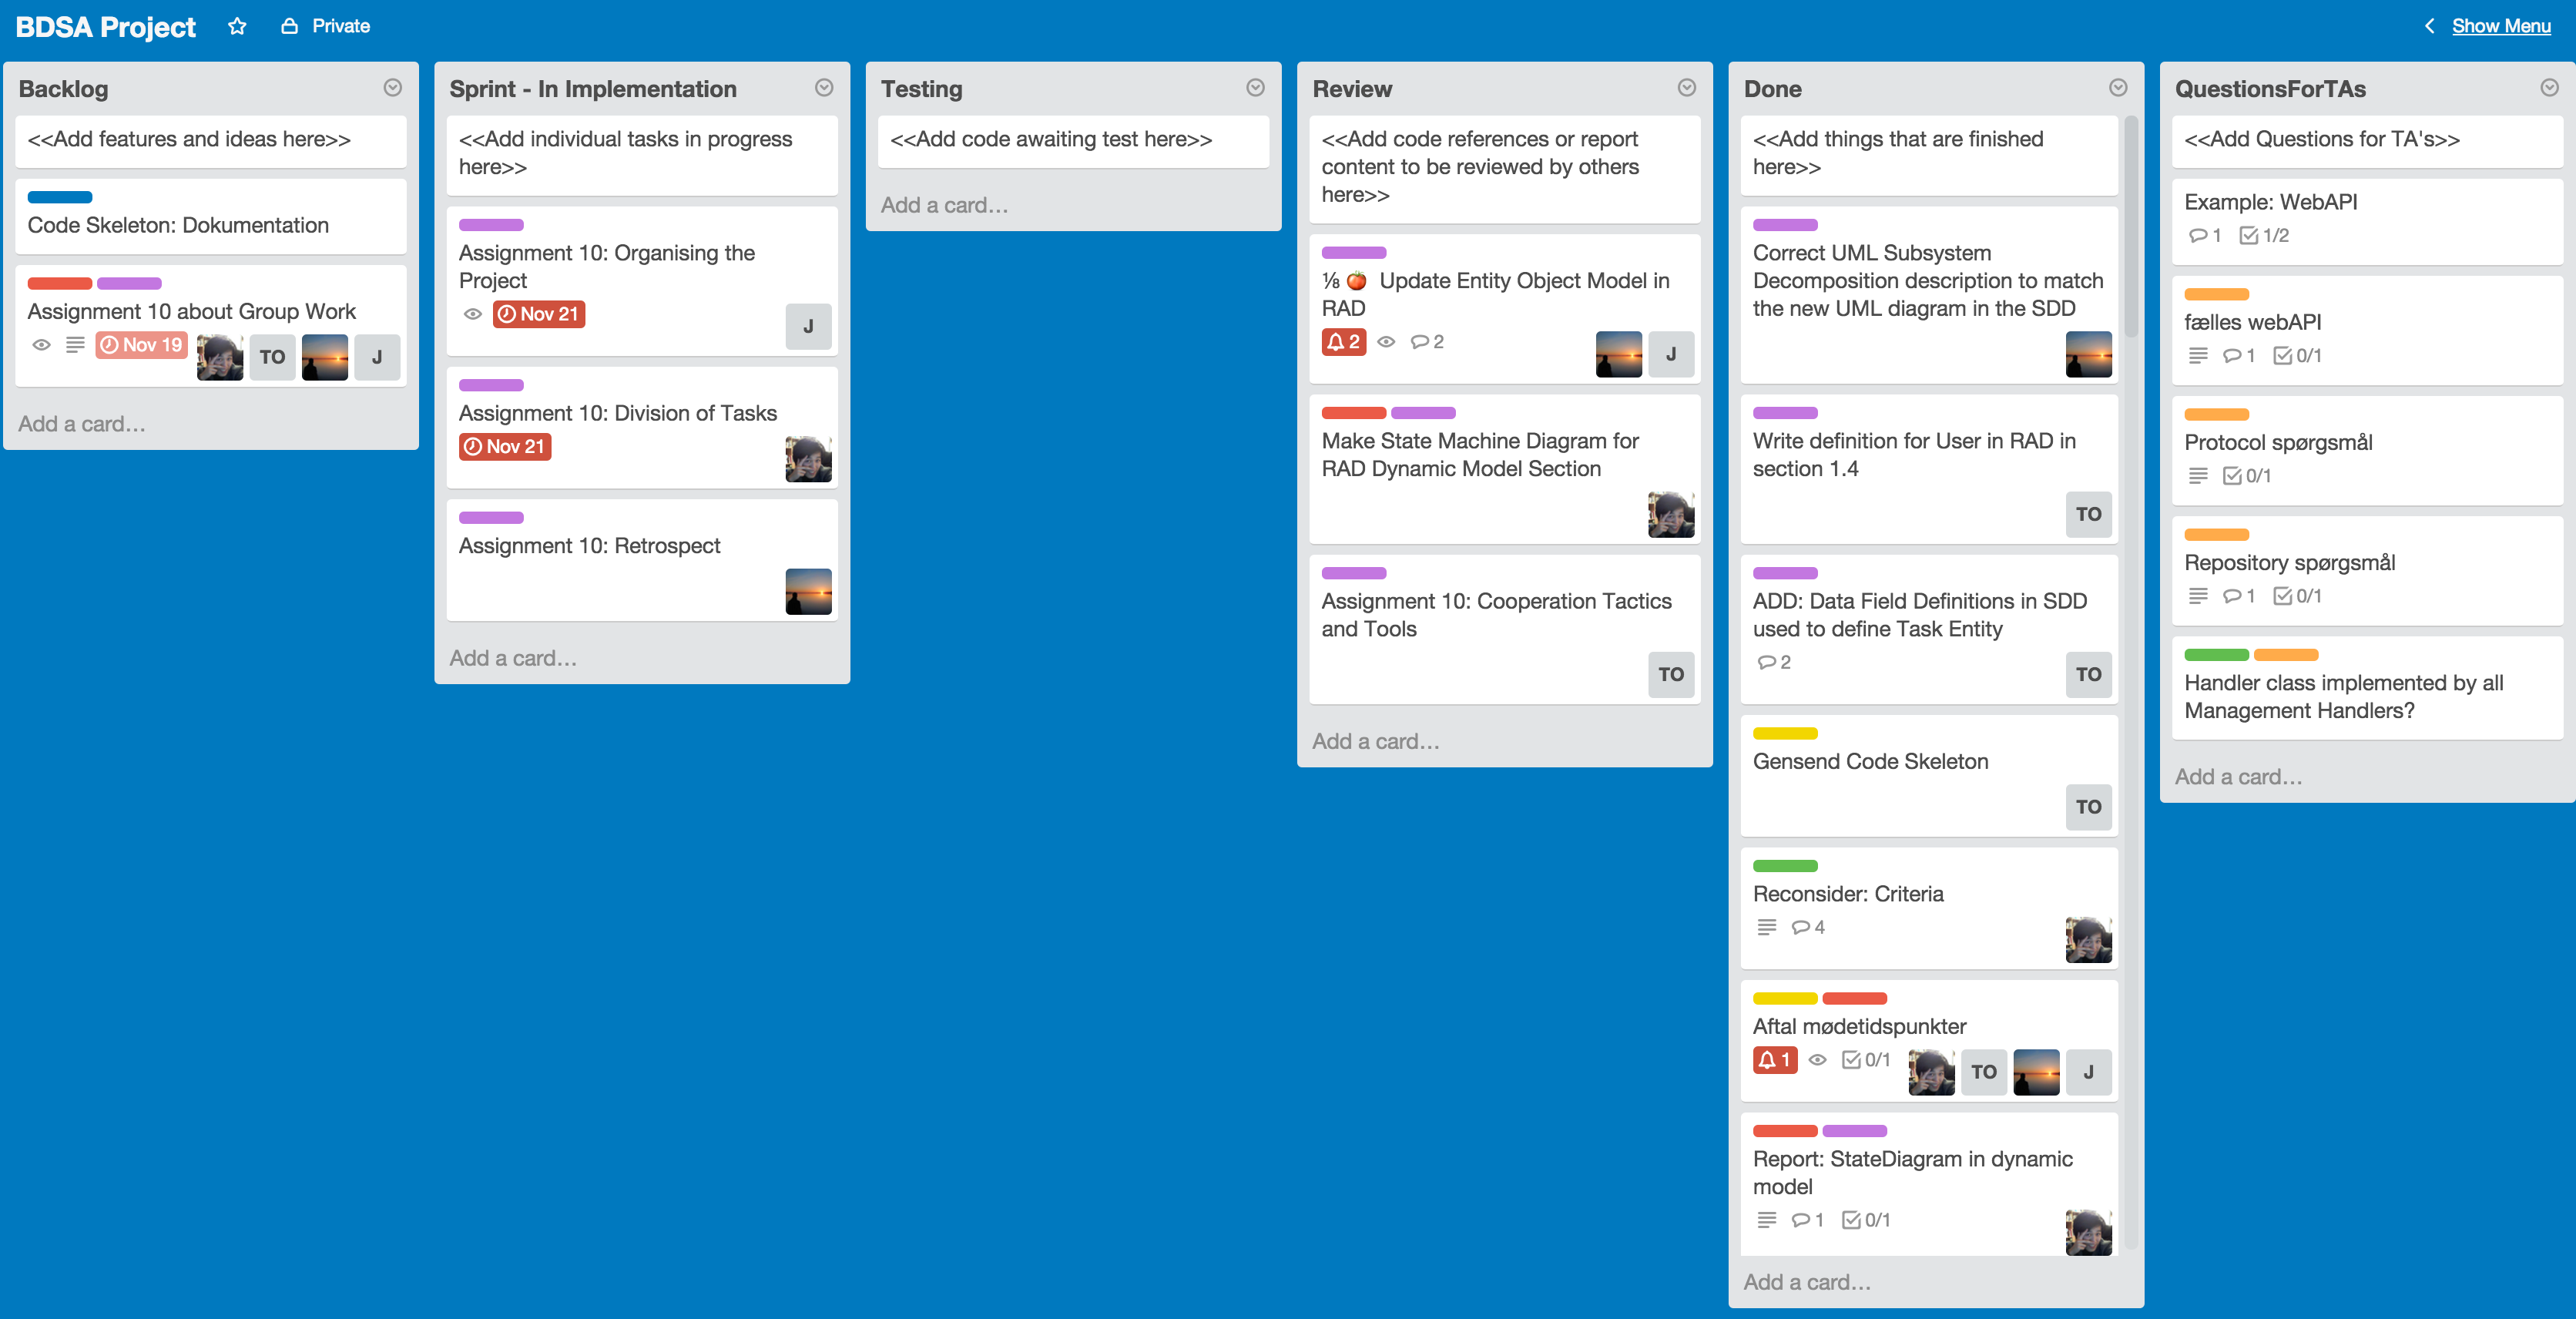
\includegraphics[width=10cm]{Taskboard}
	\caption{An example of our taskboard}
	\label{fig:rad}
\end{figure}